The goal of image restoration, detached from a specific noise model, is to estimate the latent\footnote{\textit{Latent} variables are unobserved and can only be inferred from the observed data.} clean image $Y$, from an incomplete or corrupted (noisy) image $X$ where

\begin{equation}\label{eq:images}
    Y, X \in \mathbb{R}^{n_1 \times n_2 \times \cdots \times n_d}
\end{equation}

are both $d$-dimensional discrete real-valued images.

The voxel values (intensity or counts) of noisy $X$ and latent clean $Y$ images is denoted as $x_{\mathbf{i}}$ and $y_{\mathbf{i}}$, respectively, with

\begin{equation}
    x_{\mathbf{i}}, y_{\mathbf{i}} \quad \text{for} \quad \mathbf{i} \in \mathcal{I}.
\end{equation}

where $\mathcal{I}$, the index set in the $d$-dimensional space, is defined as

\begin{equation}
    \mathcal{I} = \{[i_1, i_2, \dots, i_d]^T \mid i_1 \in [1, n_1], i_2 \in [1, n_2], \dots, i_d \in [1, n_d]\}
\end{equation}

\todo[disable]{It's always good to state where objects come from, i.e., in which spaces they are. Here it could be $Y\in\mathbb{R}^{n_1\times\cdot\times n_d}$ if $Y$ is a $d$-dimensional discrete real valued image.}
\todo[disable]{$\in$?}
\todo[disable]{This kinds of reverses the logic. Before you can connect the observation $X$ to the true image $Y$, you first need to define exactly what the true image $X$ is supposed to be. From the above I would say it's a d-array of real values.}
\todo[disable]{$\in$? In any case, the set of all possible indices should have a name, e.g., $\mathcal{I}$.}

\todo[disable]{From where to where does $\mathcal{F}$ map? Also, this does not seem very general, since this $\mathcal{F}$ is limited to operate pixel-wise and cannot take into account the position $\mathbf{i}$ at all. It still may be general enough for what you need though. I don't know yet, since I just started reading.}
In the most general form, the observation model can be defined as $X$ being a mapping of $Y$ through a function $\mathcal{F}$, which is generally stochastic. This can be written as:\todo[disable]{Will you give examples for $\mathcal{F}$ later? I think it would already be a good place to have a very simple example right here, e.g. additive noise. Then we probably see, that this is not truly a function, but involves a random variable.}
\begin{equation}\label{eq:observation-model}
    X = \mathcal{F} (Y)
\end{equation}
where $\mathcal{F}$ can vary depending on the noise model (e.g., additive or multiplicative noise, etc.), or other corruptions such as blurring, distortions etc. \todo[disable]{To understand that, you should put an example $\mathcal{F}$ here. I'm not completely sure how you mean this exactly.}

One widely used model is additive noise model, where the function $\mathcal{F}(Y)$ simply adds noise $N$ to the clean image $Y$. In this case, the observation model can be written as:
\begin{equation}\label{eq:observation-model-additive}
    X = Y + N
\end{equation}
\todo[disable]{This does not fit into your framework for the mapping $\mathcal{F}$, because this does not do the same at every pixel: At pixel $\mathbf{i}$, the noise $n_\mathbf{i}$ is added, but this depends on $\mathbf{i}$.}

where the common assumption for $N$ is \gls{AWGN}, normal distributed $\mathcal{N}$ with mean \num{0} and variance $\sigma^2$
\begin{equation}\label{eq:awgn}
    N \sim \mathcal{N}(0, \sigma^2)
\end{equation}
\todo[disable]{This equation seems to be incomplete, $\mathcal{N}(0, \sigma^2)$ (make sure you have defined this notation) is a scalar valued distribution, but the way you use $N$, it must be a matrix, where every entry of that matrix is drawn independently from $\mathcal{N}(0, \sigma^2)$.}

The inverse problem, of image restoration\footnote{Depending on context, also referred to as reconstruction or denoising.}, to estimate $Y$ from $X$, is an \textit{ill-posed} problem; meaning that there are multiple possible solutions of the estimated image $\hat{Y}$ that are not unique or equal to the true image $Y$. This is due to the loss of information during the observation process, leading to an under-determined system. Depending on the prior knowledge posed, different estimates of the latent clean image can be recovered.

In the following chapter, we shall look at an \gls{AWGN} denoising algorithm--the celebrated \gls{BM3D}, introduced first by \citeauthor{dabovImageDenoisingSparse2007} in \cite{dabovImageDenoisingSparse2007}, building upon many of the classical denoising techniques such as transform domain denoising, filtering methods (such as the Wiener filter) and \gls{NLM}. We will look at a noise model for Poisson distributed data, discussing the Anscombe \gls{VST} for stabilizing its variance, the inversion of the transform, and the \gls{BM3D} algorithm for Poisson noise.

\section{Image Denoising in Spatial and Transform Domains}
Image restoration techniques have been explored in both the spatial and transform domains\todo[disable]{Directly give an example for what transform domains are, e.g., the frequency domain.} \cite{buadesReviewImageDenoising2005,diwakarReviewCTImage2018}. For instance, the Fourier transform is commonly used to map images to the frequency domain. A simple way of denoising in this transform domain is to filter out the high frequency components that typically represent noise elements, followed by an inverse Fourier transform. Other transforms include wavelet transforms, discrete cosine transforms, and curvelet transforms.

In the spatial domain, several linear and nonlinear filtering techniques exist, utilizing different kernels to perform direct manipulation on pixel values. Linear filters, such as the mean filter, compute the\todo[disable]{inserted ``weighted''} weighted average of pixel values in a neighborhood and, in doing so, smooth the image but usually result in edge blurring. Another popular linear filter is the Gaussian filter, which applies a Gaussian kernel to the image to perform smoothing.
\todo[disable]{This short literature overview needs references that back your statements.}

\subsection{Wiener Filter}
\todo[disable]{Would be nice to have more details on the Wiener filter here. This is used in BM3D, so it's highly relevant.}
Wiener filtering is a transform domain restoration technique operating on statistical principles. Based on the additive noise model defined in \cref{eq:observation-model-additive}, it aims to minimize the \gls{MSE} between the estimated $\hat{Y}$ and latent clean image $Y$, which can be written as:

\begin{equation}\label{eq:wiener-mse}
    \hat{Y} = \arg \min_{\hat{Y}} \mathbb{E} \left[ \| Y - \hat{Y} \|^2 \right]
\end{equation}

This formulation is a case of risk minimization, a concept discussed in \cref{ch:deep_learning} in the context of learning algorithms. The noisy signal $X$ can be expressed in the frequency domain (Fourier basis) using the Fourier transform $\mathfrak{F}$ as:

\begin{equation*}
    X(f) = \mathfrak{F}(X)
\end{equation*}

where $f$ is the frequency. The Wiener filter $H(f)$ is then expressed as a linear filter that scales each frequency component of the observed signal based on the \glspl{PSD} of $Y$ and $N$: 

\begin{equation*}
H(f) = \frac{S_Y(f)}{S_Y(f) + S_N(f)}
\end{equation*}

with $S_Y(f)$ and $S_N(f)$ the \gls{PSD} of latent image $Y$ and noise $N$, respectively. The most common Wiener filtering technique assumes the \gls{PSD} of $N$ to be constant, which is the case for \gls{AWGN}. However, usage of other additive noise priors is as easy as changing the \gls{PSD} of $N$.

This (optimal) filter $H(f)$, based on image properties, can be applied to $X(f)$ to estimate the latent clean image in the frequency domain:

\begin{equation*}
    \hat{Y}(f) = H(f) X(f)
\end{equation*}

and this can be transformed back to the spatial domain to obtain a denoised estimate

\begin{equation*}
    \hat{Y} = \mathfrak{F}^{-1}(\hat{Y}(f))
\end{equation*}

Notice from above that the Wiener filter requires access to the latent clean image $Y$ to compute $S_Y(f)$, which is generally not available. Hence, empirical Wiener filters\footnote{This then becomes a case of empirical risk minimization.}, based on noisy $X$, were proposed by \citeauthor{yaroslavskyDigitalPictureProcessing1985} \cite{yaroslavskyDigitalPictureProcessing1985}. The method follows a moving window approach, where the filtering is estimated from the local statistics of the image. The filter is then applied to the central pixel of the window and inverted to estimate the latent clean image.

As the Fourier basis operates globally, applying Wiener filtering with this basis can introduce periodic artifacts, as global transforms may overemphasize large-scale image features and fail to capture fine local details. This limitation has motivated the development of local adaptive variants and the exploration of alternative transform domains such as wavelets, which better capture local image characteristics \cite{buadesReviewImageDenoising2005}.

\subsection{Non-Local Means}
\todo[disable]{Since NLM is quite related to BM3D, it would also be helpful to define this in detail here. The definition is not that involved and I would say quite instructive to understand the non-locality.}
\todo[disable]{``also''? What else uses this redundancy? BM3D, but you haven't mentioned that one yet. At leae not in this chapter.}

Other than linear filters, non-linear filters such as the median filter, replace each pixel with the median value of its neighbors and are much better at removing salt-and-pepper noise. Other approaches, such as bilateral filtering, combine spatial proximity and intensity similarity, allowing for selective smoothing that  preserves sharpness around edges. 

The principle behind \gls{NLM} denoising builds on the redundancy of similar patches in the image and estimates a pixel value by taking a weighted average over other pixels with a similar local structure, regardless of their spatial distance. By utilizing these priors, denoising algorithms can indeed aggressively use the intrinsic properties of the images and thereby enhance the visual quality and provide estimates closer to the latent clean image.

Non-Local Means (NLM) denoising is a highly effective method for removing noise by leveraging the inherent redundancy found in natural images. Unlike local filters, which operate on immediate pixel neighborhoods, NLM uses a non-local approach, meaning that it searches the entire image for patches or neighborhoods that resemble the local structure of a pixel's neighborhood, regardless of their spatial distance. The algorithm replaces a noisy pixel by computing a weighted average of all pixels in the image, with the weights determined by the similarity of their neighborhoods.

The similarity between the neighborhoods of pixels $i$ and $j$ is measured using the Gaussian-weighted Euclidean distance between intensity vectors in a window surrounding each pixel:

\begin{equation}
    w(i,j) = \frac{1}{x(i)} \exp \left( -\frac{\|v(\mathcal{N}_i) - v(\mathcal{N}_j)\|_{2,a}^2}{h^2} \right),
\end{equation}

where $v(\mathcal{N}_i)$ is the vector of pixel intensities within the neighborhood $\mathcal{N}_i$ of pixel $i$, and $h$ is a parameter controlling the decay of weights as a function of this distance. The normalization factor $x(i)$ ensures that the weights sum to 1 for each pixel $i$.

NLM is particularly effective at preserving edges and textures in the image, as the weight $w(i,j)$ assigns higher values to pixels whose neighborhoods are similar in appearance to the target pixel's neighborhood. As a result, NLM performs well in removing noise while maintaining important image features, making it a popular choice for denoising tasks, especially when the noise is uniformly distributed across the image.


\section{BM3D: Denoising in Sparse Domain}

\begin{figure}
    \centering
    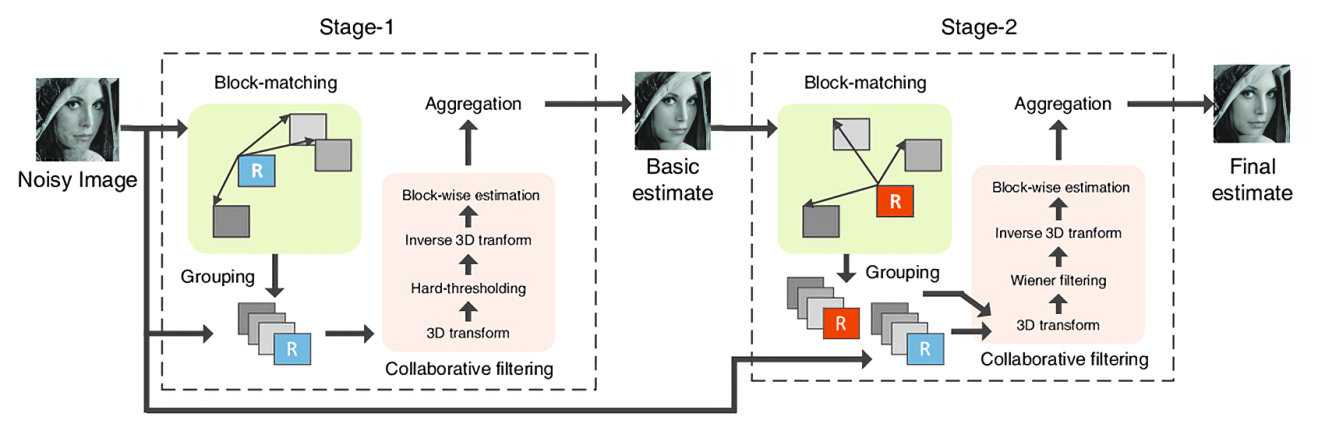
\includegraphics[width=1\linewidth]{images/bm3d_schematic.png}
    \caption{Block diagram showing the 2-stage \gls{BM3D} algorithm, consisting of block matching, collaborative filtering, and aggregation. Reprinted from \cite{wangFPGABasedHardwareAccelerator2020}, under the terms of the Creative Commons Attribution 4.0 International License.}
    \label{fig:bm3d-schematic}
\end{figure}


As shown in \cref{alg:bm3d} and \cref{fig:bm3d-schematic}
\todo[disable]{This needs more details. Try to provide the essential formulas of what is actually computed for all steps. You don't need to put those details into the algorithm, it's better to add them to the main text.}
, the \gls{BM3D} scheme works by grouping similar patches in a 2D image and applying a 3D transform\footnote{This algorithm has also been proposed for 3D images, dubbed BM4D \cite{mNonlocalTransformdomainFilter}.}. This leads to an enhanced sparse representation of the image which after filtering is transformed back to the spatial domain.
% Main BM3D Algorithm
\begin{algorithm}
    \caption{BM3D Denoising Algorithm}\label{alg:bm3d}
    \begin{algorithmic}[1]
    \Require Noisy image $X$, noise variance $\sigma^2$
    \Ensure Denoised image $\hat{Y}$
    \Statex
    \Procedure{BM3D}{$X$, $\sigma^2$}
        \State $\hat{Y} \gets X$
        
        \For{each reference block $B_R$ in $X$}
            \State $B_{G} \gets \textsc{BlockMatching}(B_R, X)$
            \State $B_{F} \gets \textsc{CollaborativeFiltering}(B_{G}, \sigma^2)$
            \State \textsc{Aggregate} $B_{F}$ into $\hat{Y}$
        \EndFor
        
        \State \textbf{return} $\hat{Y}$
    \EndProcedure
    \end{algorithmic}
\end{algorithm}

In the Grouping step, candidate blocks $B_i$ which are the least dissimilar to an $N_1 \times N_1$ reference block $B_R$ are grouped together using the normalized $l^2$-distance as dissimilarity measure:

$$d(B_R, B_i) = \frac{\|B_R - B_i\|_2^2}{N_1^2}$$

with group $B_G$ formed by selecting blocks that have distance below the threshold $\tau$:

$$B_G = \{ B_i : d(B_R, B_i) \leq \tau \}$$

The Collaborative Filtering\footnote{Interestingly, collaborative filtering has been the backbone of recommendation systems such as by Netflix and Spotify \cite{bellLessonsNetflixPrize2007,drorYahooMusicDataset2012}.}\todo[disable]{Reference for the Netfilx/Spotify statement?} shown in \cref{alg:collaborativefiltering} is then applied to the grouped blocks. This step consists of a 3D transform such as the discrete cosine transform (or the wavelet transform can be used).
\todo[disable]{This 3D stacking and 3D filtering is a crucial component, which should be elaborated / illustrated more.}
A filter is applied to the transformed blocks to remove noise, initially by hard thresholding and in the second run by Wiener filtering. The inverse 3D transform is then applied to the filtered blocks, and the filtered blocks are aggregated to form the estimate. The first run is considered the basic estimate, and it is only after Collaborative Wiener filtering that the final estimate is obtained.
\todo[disable]{One a coarse level, this is all correct, but I would put much more detail. Also a sketch would be helpful.}
    
% Collaborative Filtering Algorithm
\begin{algorithm}
    \caption{Collaborative Filtering}\label{alg:collaborativefiltering}
    \begin{algorithmic}[1]
    \Require Group of similar blocks $B_{G}$, noise variance $\sigma^2$
    \Ensure Filtered block $B_{F}$
    \Procedure{CollaborativeFiltering}{$B_{G}$, $\sigma^2$}
        \State $B_{T} \gets \textsc{3DTransform}(B_{G})$
        \State $B_{F} \gets \textsc{ApplyFiltering}(B_{T}, \sigma^2)$
        \State $B_{I} \gets \textsc{Inverse3DTransform}(B_{F})$
        \State Aggregate $B_{I}$ into $B_{F}$
        \State \textbf{return} $B_{F}$
    \EndProcedure
    \end{algorithmic}
\end{algorithm}

The \gls{BM3D} algorithm had showed one of the best denoising performances and can only be contested by the recent deep-learning based denoising methods. 

\section{Poisson Noise and Variance Stabilization}\label{sec:poisson-noise-model}
In imaging systems, the observed intensity $x_{\mathbf{i}}$ at each voxel $\mathbf{i}$ of a noisy image $X$ is a stochastic mapping of the latent distribution $y_{\mathbf{i}}$ due to the measurement process.\todo[disable]{The fact that this is a stochastic mapping is not due to the low light setting. For that it's enough that you are measuring. The Possion part is due to the low light setting.} In low light settings, such as photon-limited imaging, $x_{\mathbf{i}}$ can be modeled as independent Poisson characterized by the true intensity $y_{\mathbf{i}}$, we aim to estimate\footnote{This assumption is discussed in more detail in \cref{section:photoelectron-counting-stats}, and is true for a constant intensity light source.} \cite{makitaloOptimalInversionAnscombe2011,kimDeepLearningbasedStatistical2021} 
\begin{equation*}
    x_{\mathbf{i}} \sim \text{Poi}(y_{\mathbf{i}})
\end{equation*}

where $\text{Poi}(y)$ denotes the Poisson distribution with parameter (and latent intensity) $y$. 

To simplify notation moving forward, we denote the observed value as $x$ and the underlying intensity as $y$. Using this, we can express the \gls{PMF} of $x$ given $y$  as:

\begin{equation}\label{eq:poisson-pmf-1}
    P(x = k| y) = \frac{y^k e^{-y}}{k!} , \quad k \in \mathbb{N}_0
\end{equation}

Poisson distribution has the key property that the mean and variance are equal, $\mathbb{E}[x\mid y] = \text{Var}[x\mid y] = y$, with standard deviation $\sqrt{y}$. In contrast to the \gls{AWGN} model, which assumes a variance independent of the true intensity, the Poisson noise model has variance scaling with the true intensity. This implies that with decreasing intensity, the fluctuations (standard deviation) increase. Consequently, \gls{AWGN} denoising algorithms, such as \gls{BM3D}, can not directly be applied to Poisson noise.

\subsection{Variance Stabilizing Transformations}
To address this issue, suitable transformations that stabilize the variance, making it largely independent of the mean (similar to the normal distribution) can be beneficial. Transforms such as these are known as \glsxtrfullpl{VST}. \citeauthor{bartlettSquareRootTransformation1936} \cite{bartlettSquareRootTransformation1936} first showed such a transform: the square root transformation $T_1$:
%Moreover, \glspl{VST} variance stabilization is independent of the sample size.

\begin{equation}
    T_1: [0, \infty) \to [0, \infty), \quad x \to \sqrt{x}
\end{equation}

where we look at a Poisson variable $x \sim \text{Poi}(y)$.

\begin{figure}
    \centering
    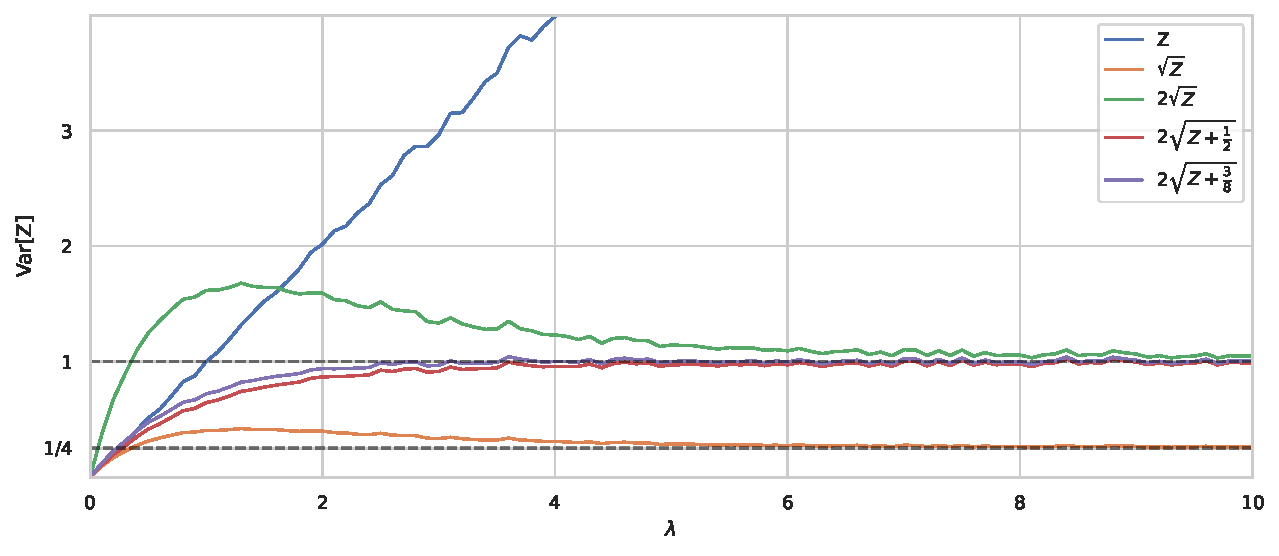
\includegraphics[width=1\linewidth]{images/data_transform_anscombe.pdf}
    \caption{\textit{Variance stabilization through various transformations of Poisson-distributed data.} The plot shows the variance of Poisson variables (blue) along with the variances of their transformed values under different variance-stabilizing transformations: the square root transform ($T_1(x)$, scaled $2T_1(x)$), the square root transform with a constant of $\frac{1}{2}$ ($T_2(x)$, scaled $2T_2(x)$), and the Anscombe transform ($T_A(x)$). 
    As the Poisson parameter $y$ increases, the variance of the scaled transforms stabilizes to approximately $1$, with the fastest convergence using the Anscombe transform.
    The scaling by $2$ allows the data to more closely approximate a standard normal distribution. Dashed horizontal lines indicate the stabilization levels.}
    \label{fig:data-transform-anscombe}
\end{figure}

Applying this transform to Poisson data makes the transformed values approximately normally distributed as the Poisson parameter $y$ increases. The variance of Poisson variable $x$ (blue) and transformed variable using $T_1$ (orange) as a function of $y$ can be seen in \cref{fig:data-transform-anscombe}, with the variance of $\sqrt{x}$ stabilizing to $\frac{1}{4}$ with increasing $y$. \citeauthor{bartlettSquareRootTransformation1936} additionally showed that by adding a constant of $\frac{1}{2}$ to the square root transform, the convergence to normality improves, leading to the transformation:

\begin{equation}
    T_2: [0, \infty) \to [0, \infty), \quad x \to \sqrt{x + \frac{1}{2}}
\end{equation}

$T_2$ (red) in \cref{fig:data-transform-anscombe} shows this faster convergence (also preventing overshoot) when compared to the $T_1$ (orange). $T_1$ (purple) and $T_2$ (green) are also shown scaled by \num{2}, effectively centering the variance\footnote{The variance scales by square of the scaling factor, i.e., $\text{Var}[aZ] = a^2 \text{Var}[x]$} around \num{1}, yielding a transformed variable that approximates a standard normal distribution.

\citeauthor{anscombeTransformationPoissonBinomial1948} \cite{anscombeTransformationPoissonBinomial1948} further showed that using the  constant of $\frac{3}{8}$ is an optimal \gls{VST} $T_A$ for Poisson distributed data:

\begin{equation}\label{eq:anscombe-transform}
    T_A: [0, \infty) \to [0, \infty), \quad x \to 2 \sqrt{x + \frac{3}{8}}
\end{equation}

Comparing scaled $T_2$ (purple) with $T_A$ (black) in \cref{fig:data-transform-anscombe}, it can be seen that the variance of the Anscombe transform stabilizes to \num{1} faster, while not significantly different from the $T_2$. \cref{fig:hist-anscombe} provides an alternate visualization showing the distributions at different $y$ before and after applying $T_A$. As $y$ increases, the variance of the transformed data $Var[T_A(x)]$ stabilizes to $1$, along with a bias in the expected value $\mathbb{E}[T_A(x)]$.

\begin{figure}
    \centering
    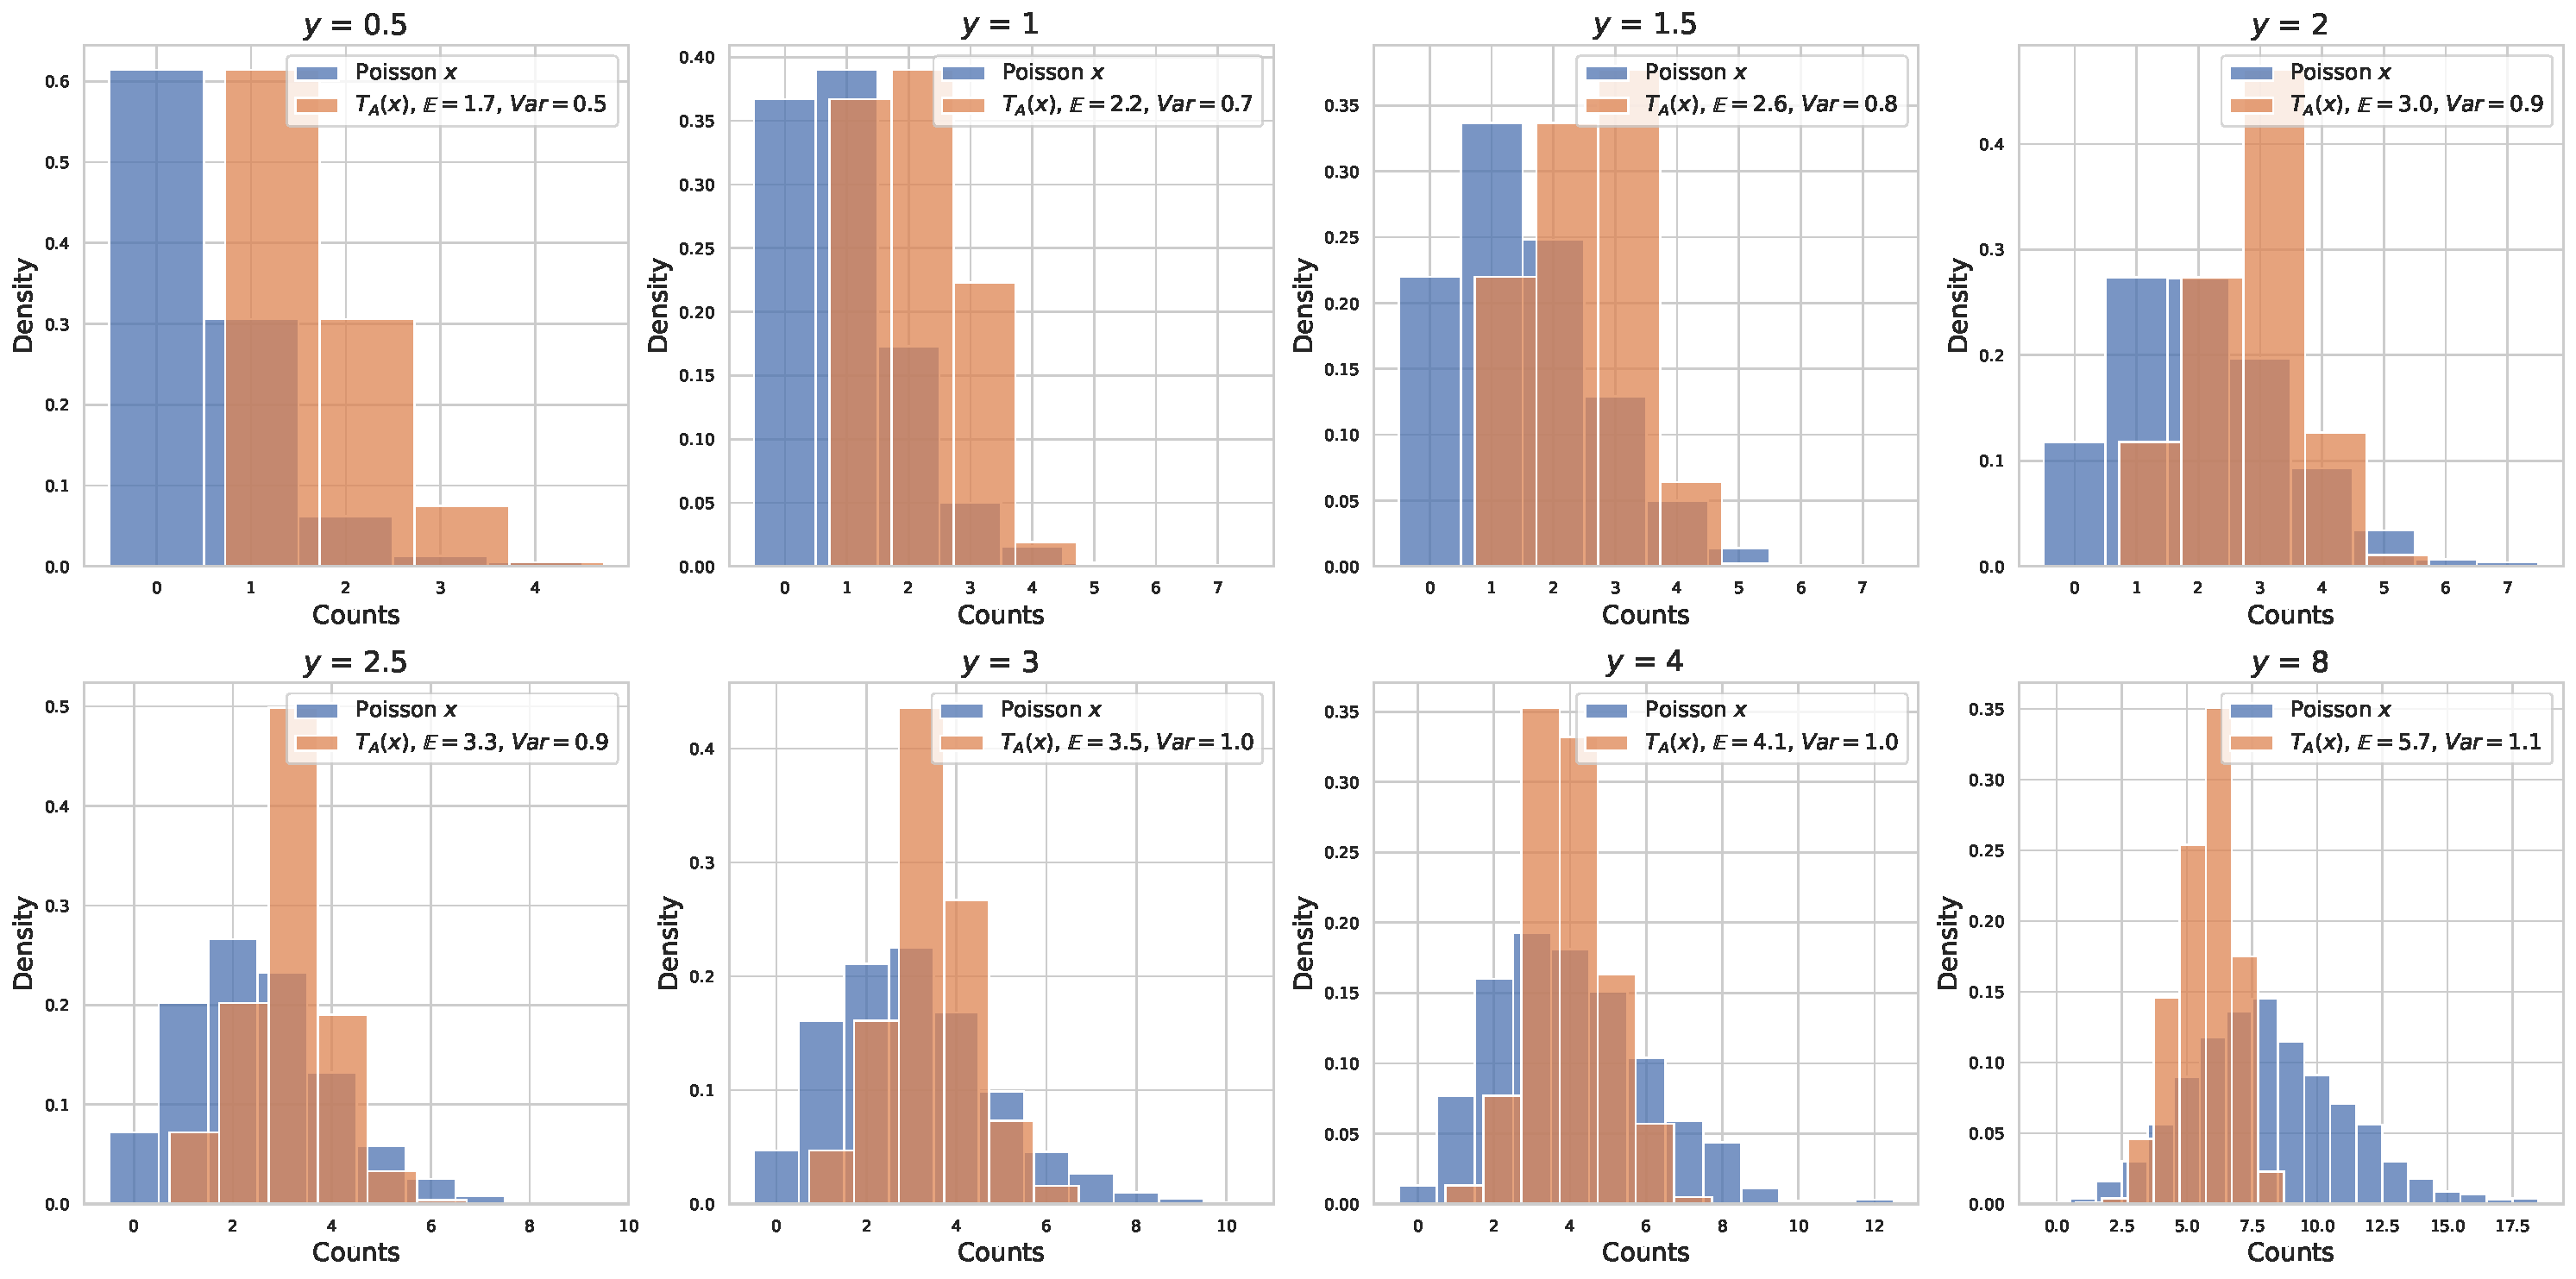
\includegraphics[width=1\linewidth]{images/hist_anscombe.pdf}
    \caption{\textit{Variance stabilization through the Anscombe transform.} The histogram shows the empirical distribution of Poisson  variables with different $y$ values (\numlist{0.5;1;1.5;2;2.5;3;4;8}), both before ($x$) and after applying the Anscombe transform ($T_A(x)$). The expected value $\mathbb{E}[T_A(x)]$ and variance $\text{Var}[T_A(x)]$ of the transformed data are shown in the legend, with the variance stabilizing to \num{1} as $y$ increases. It can also be seen that expected value presents a bias after the transformation that should be corrected when applying the inverse transform.}
    \label{fig:hist-anscombe}
\end{figure}

\subsection{Inverse Transformations}
The Anscombe transform $T_A$ can hence be applied to a noisy pixel $x$ (described as $x \sim \text{Poi}(y)$) to stabilize the variance, making it suitable for denoising using \gls{AWGN} denoising algorithms. After applying $T_A$ and denoising, we obtain an estimate $d$ that approximates $\mathbb{E}[T_A(x) \mid y]$. The challenge lies in finding an appropriate inverse transformation to recover an estimate of the latent intensity $y$. 

To this end, consider the algebraic inverse of $T_A$, written as:

\begin{equation}
    I_A: [0, \infty) \to [0, \infty), \quad d \to \left(\frac{d}{2} \right)^2 - \frac{3}{8}
\end{equation}

Due to the non-linearity of the Anscombe transform:
\begin{equation*}
    \mathbb{E}[T_A(x) \mid y] \neq T_A(\mathbb{E}[x \mid y])
\end{equation*}

and therefore

\begin{equation*}
    I_A(\mathbb{E}[T_A(x) \mid y]) \neq \mathbb{E}[x \mid y] = y
\end{equation*}

meaning that $I_A$ provides a biased estimate of $y$, as illustrated in \cref{fig:anscombe-expectation-inversion}\footnote{Note that this Figure is similar to Figure~1 in \cite{makitaloOptimalInversionAnscombe2011}, where they present the estimate of $y$ against the transformed and denoised variable $d$. The author finds that plotting against the Poisson parameter $y$ is simpler to understand.}. In this figure, $I_A(d)$ (green line) diverges from the mean $\mathbb{E}[x]$ (dashed blue line) for all values of $y$. 

To reduce this bias, \citeauthor{anscombeTransformationPoissonBinomial1948} \cite{anscombeTransformationPoissonBinomial1948} proposed an inversion $I_B$ that is asymptotically unbiased:

\begin{equation}
    I_B: [0, \infty) \to [0, \infty), \quad d \to \left(\frac{d}{2} \right)^2 - \frac{1}{8}
\end{equation}

The asymptotic unbiasedness of $I_B$ can also be seen in \cref{fig:anscombe-expectation-inversion} (red line), as when $y \geq 3$ (high-counts), the expected value of $I_B(d)$ is close to $y=\mathbb{E}[x]$. However, for low-counts, the bias is even higher than the algebraic inverse.

\begin{figure}
    \centering
    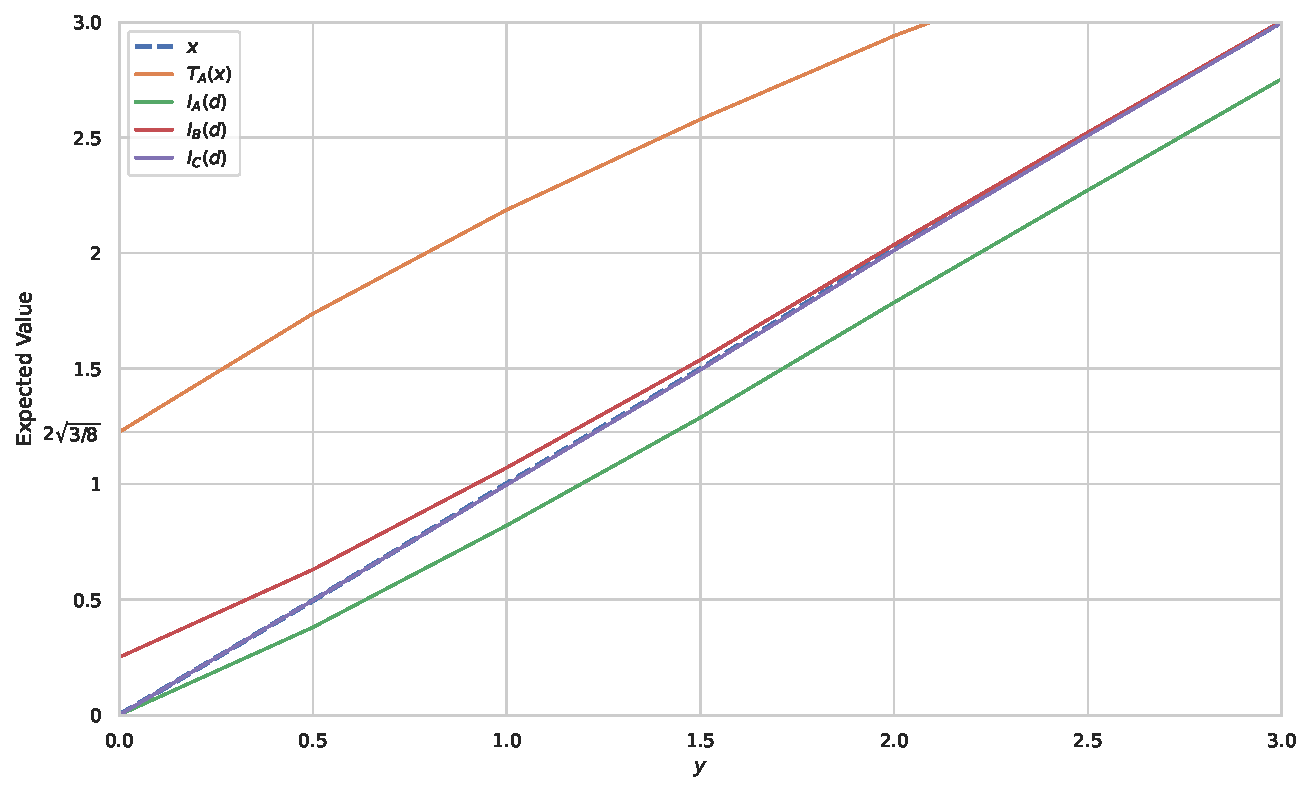
\includegraphics[width=1\linewidth]{images/anscombe_expectation_inversion.pdf}
    \caption{\textit{Different inversions of Anscombe transformed data to estimate the true value.} This plot illustrates the estimates of $y$ as a function of the Poisson parameter $y$. The estimates for $y$ are obtained by inverting the Anscombe transform using three different methods: the algebraic inverse ($I_A$, green), the asymptotically unbiased inverse ($I_B$, red), and the exact unbiased inverse ($I_C$, purple). The expected value of $x$ (dashed blue), $\mathbb{E}[x]=y$ and Anscombe transform $T_A(x)$ (orange) are also shown for reference.}
    \label{fig:anscombe-expectation-inversion}
\end{figure}


To address these limitations, \citeauthor{makitaloOptimalInversionAnscombe2011} introduced an exact unbiased inverse, meaning it produces a mapping $I_C$ that satisfies:

\begin{equation}
    I_C: \mathbb{E}[T_A(x) \mid y] \to \mathbb{E}[x \mid y] = y
\end{equation}

To construct such an exact unbiased inverse $I_C$, the expected value of the Anscombe-transformed variable, $\mathbb{E}[T_A(x) \mid y]$, which reflects the expected value of $T_A(x) $ (where $x \sim Poi(y)$) is given by

\begin{equation}   
    \mathbb{E}[T_A(x) \mid y] = \sum_{x=0}^{\infty} T_A(x) \cdot P(x \mid y),
\end{equation}

where $T_A(x)$ is defined in \cref{eq:anscombe-transform}, and $P(x \mid y)$ in \cref{eq:poisson-pmf-1}, so we substitute this into the expectation:

\begin{equation*}
    \mathbb{E}[T_A(x) \mid y] = \sum_{x=0}^{\infty} 2 \sqrt{x + \frac{3}{8}} \cdot y^x e^{-y} \frac{1}{x!}
\end{equation*}

This expectation sums over all possible values of $x$, weighting each transformed value $T_A(x)$ by its probability under the Poisson distribution with mean $y$. Calculating this expectation accurately allows the exact unbiased inverse  $I_C$  to achieve its goal: matching the expected value of the transformed variable $T_A(x)$ back to the original mean, $y$. $I_C$ can be computed using a numerical optimization algorithm, as detailed in \cite{makitaloOptimalInversionAnscombe2011}. 

The authors additionally find that the maximum likelihood inversion\footnote{They also find a minimum \gls{MSE} inversion that coincides with $I_C$ when the denoising is successful i.e. the true mean is recovered.} coincides with $I_C$. This method is also shown to perform better than the asymptotically unbiased inverse $I_B$ and the algebraic inverse $I_A$ \cite{makitaloOptimalInversionAnscombe2011}, and is hence the inversion we use in the rest of this work.

A closed form approximation of $I_C$ is also available in \cite{makitaloClosedFormApproximationExact2011}, written as:

\begin{equation}
    I_D(d) = \frac{1}{4} d^2 + \frac{\sqrt{\frac{3}{2}}}{4} d^{-1} - \frac{11}{8} d^{-2} + \frac{5 \sqrt{\frac{3}{2}}}{8} d^{-3} - \frac{1}{8}
\end{equation}

\subsection{The Anscombe BM3D Algorithm}
Poisson corrupted 2D images can hence be denoised using a three-step scheme shown in \cref{fig:anscombe-bm3d}; Applying the Anscombe transform to noisy image $X$, denoising the transformed image the \gls{BM3D} algorithm, and inverting the transformation to obtain estimate $\hat{Y}$ of the latent clean image $Y$. We use the Anscombe transform $T_A$ and the exact unbiased inversion $I_C$ for the pixel-wise transformations in the image. An algorithmic scheme can be seen in \cref{alg:anscombe-bm3d}, where we assume that $T_A$ and $I_C$ can take an image as an input.

This method has been shown to perform better than methods based on explicit Poisson noise removal \cite{makitaloOptimalInversionAnscombe2011}. Therefore, in the next chapter we make use of the scheme described in \cref{fig:anscombe-bm3d} to denoise 2D images from \gls{MPES} datasets.

% create figure with bm3d_anscombe_scheme.pdf
\begin{figure} 
    \centering
    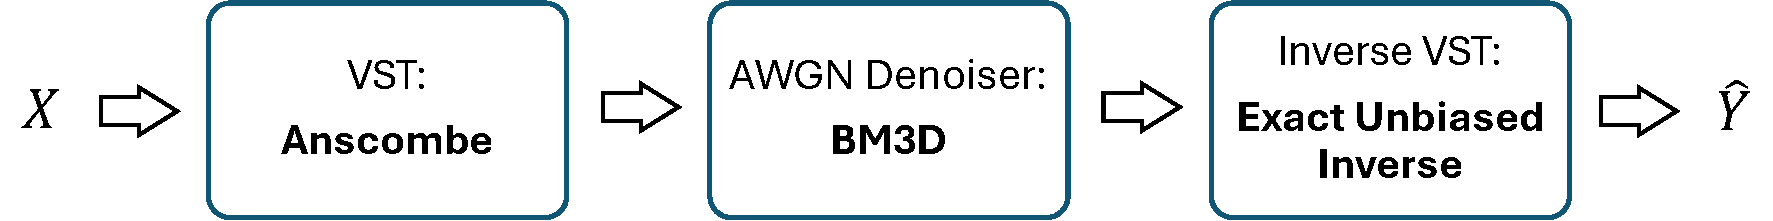
\includegraphics[width=1\linewidth]{images/bm3d_anscombe_scheme.pdf}
    \caption{Block diagram showing the denoising scheme for Poisson corrupted images, consisting of the Anscombe transform, BM3D denoising, and the inversion of the Anscombe transform.}
    \label{fig:anscombe-bm3d}
\end{figure}

\begin{algorithm}
    \caption{Algorithm to Denoise Poisson Corrupted Images}\label{alg:anscombe-bm3d}
    \begin{algorithmic}[1]
    \Require Noisy image $X$
    \Ensure Denoised image $\hat{Y}$
    \Statex
    \Procedure{AnscombeBM3D}{$X$, $\sigma^2$}
        \State $X_{\text{A}} \gets T_A(X)$
        
        \State $D \gets \textsc{BM3D}(X_A, \sigma^2)$
        
        \State $\hat{Y} \gets I_C(D)$
        
        \State \textbf{return} $\hat{Y}$
    \EndProcedure
    \end{algorithmic}
\end{algorithm}


\todo[disable]{What is this voxel $X$? Do you mean $\mathbf{i}$? In any case, some more explanations would be helpful.}
\todo[disable]{How can you conclude that and what does this mean exatly? Did you introduce the stochastic terminology already?}
\todo[disable]{Why do we need the expectation to the noise?}
\todo[disable]{Is the acronym VST already defined? Those are usually spelled out at first use, not only in once in some acronym table.}\tododone[disable]{Yes it happens automatically. It's defined in the introduction of the chapter. If preferred, I can redefine here.}
\todo[disable]{It would be helpful to state that one starts here with data samples from a distribution where the variance depends on the signal (pointing to the previous section as an example).}
\todo[disable]{Stat from where to here $T$ maps, I guess it is meant to map non-negative numbers to non-negative numbers, e.g., $T:[0,\infty)\to[0,\infty),X\mapsto...$.}
\todo[disable]{Is this supposed to use an array notation? In the sense that $X$ is a 2D-array? If so, I would first state what it does with a single intensity value.}
\todo[disable]{In which sense approximately? I'd say that a plot of the variance before and after stabilization would be very illustrative here.}
\todo[disable]{Bad notation. $\mathbb{x}$ is usually the set of integers.}
\todo[disable]{I don't understand this part and what you do with the expectation here. Why is this more than just ``apply $T$, denoise, apply $T^{-1}$''?}
\todo[disable]{I don't see how the non-linearity of the transformation should result in ``an'' algebraic inverse to be asymptocically biased. It's not even clear what you mean with the term ``asymptocically biased''. For the algebraic inverse, I guess you mean by the inverse you get by solving (3.8) for $X$.}
\todo[disable]{What does ``exact unbiased'' mean?}
\todo[disable]{So the $T^{-1}$ is the ``exact unbiased inverse'', not the ``algebraic inverse''? The notation ``$T^{-1}$'' means the inverse of $T$, which is unique. If you don't apply the inverse, explain what exactly you apply, use a different notation and if possible also give a formula.}